
\documentclass{article}
\usepackage[utf8]{inputenc}


\usepackage[margin=1.1 in]{geometry}
\usepackage[T1]{fontenc}
\usepackage{mathtools}   % loads »amsmath«
\usepackage{amssymb}
\usepackage{amsfonts}
\usepackage{amsmath}
\usepackage{amsthm}
\usepackage{xcolor}
\usepackage{cancel}
%\usepackage{graphics}
\usepackage{graphicx}
%others
\usepackage{enumerate}
\usepackage{subcaption}



\usepackage{apacite}
\usepackage[round]{natbib}
%\bibliographystyle{plainnat}
\bibliographystyle{apacite}

\DeclarePairedDelimiter{\ceil}{\lceil}{\rceil}

\setlength{\parskip}{0.8em}
\usepackage{setspace}
%\singlespacing
\spacing{1.2}



\newtheorem{defin}{Definition.}
\newtheorem{teo}{Theorem. }
\newtheorem{lema}{Lemma. }
\newtheorem{coro}{Corolary. }
\newtheorem{prop}{Proposition. }
\theoremstyle{definition}
\newtheorem{examp}{Example. }
\newtheorem{problem}{}

\title{717 Metrics}
\author{Giselle Labrador Badia}
\date{March 2022}

\begin{document}

\maketitle

 Tables with standards errors are provided for all regressions and other relevant analyses that I discuss. All the Stata code pertinent to this assignment is attached. 

\begin{table}[htbp]\centering
\begin{tabular}{lc} \hline
 & (1) \\
VARIABLES & re78 \\ \hline
 &  \\
treated & 818.7* \\
 & (487.8) \\
age & -145.9 \\
 & (200.8) \\
age2 & 2.799 \\
 & (3.246) \\
educ & 206.8 \\
 & (165.5) \\
black & -1,461** \\
 & (734.3) \\
hisp & 100.5 \\
 & (958.6) \\
married & 133.9 \\
 & (660.0) \\
nodegree & -405.9 \\
 & (752.1) \\
re74 & 0.0871 \\
 & (0.106) \\
re75 & 0.0840 \\
 & (0.119) \\
Constant & 5,649 \\
 & (3,757) \\
 &  \\
Observations & 722 \\
 R-squared & 0.045 \\ \hline
\multicolumn{2}{c}{ Robust standard errors in parentheses} \\
\multicolumn{2}{c}{ *** p$<$0.01, ** p$<$0.05, * p$<$0.1} \\
\end{tabular}
\caption{OLS regression from question 1.}
\end{table}

\hspace{0.41cm} \textbf{Question 0.} I dropped the observations from the PSID comparison group. 


\hspace{0.41cm} \textbf{Question 1.} The coefficient of the treated is positive and significant and suggests that the experiment is 791.4 dollars. Although the treatment is random,  the covariates help you to get better estimates by absorbing the residual variance. You will get efficient estimates if you control for the covariates. 



\hspace{0.41cm} \textbf{Question 2.} The experimental treatment group was dropped. 

\hspace{0.41cm} \textbf{Question 3.} The table is not included but regressions results are on the log file. All the coefficients have the expected sign and are significant, except for the earning in 1974 and earning 1975 in the rich score probit regression. Only failures were completely determined in both cases (0 success).

\hspace{0.41cm} \textbf{Question 4.} Table 2 and Table 3 describes the distributions and this shows that the two groups are quite different.  Nonetheless, there is some common support, which indicates that the support condition may be satisfied. The distribution of the experimental sample is more equally distributed, while the nonexperimental distribution is shifted to the left (low propensity scores).


\begin{table}[htbp]\centering
\def\sym#1{\ifmmode^{#1}\else\(^{#1}\)\fi}
\caption{Coarse scores (pscora)}
\begin{tabular}{l*{1}{ccccccc}}
\hline\hline
          &\multicolumn{7}{c}{}                                                 \\
          &      Min&      p25&      p50&     Mean&      p75&      Max&    count\\
\hline
0         & 9.79e-13& .0000213& .0001069& .0164119& .0035243& .6872082&    15992\\
1         & .0000756& .2007289& .4716014& .3873009& .5998097& .6872082&      425\\
Total     & 9.79e-13& .0000215& .0001121& .0260134&  .003898& .6872082&    16417\\
\hline
\(N\)     &    16417&         &         &         &         &         &         \\
\hline\hline
\end{tabular}
\end{table}


\begin{table}[htbp]\centering
\def\sym#1{\ifmmode^{#1}\else\(^{#1}\)\fi}
\caption{Rich scores (pscorb)}
\begin{tabular}{l*{1}{ccccccc}}
\hline\hline
          &\multicolumn{7}{c}{}                                                 \\
          &      Min&      p25&      p50&     Mean&      p75&      Max&    count\\
\hline
0         & 2.08e-16& 1.97e-06& .0000677& .0154465& .0023622& .7886285&    15992\\
1         & 1.64e-06& .2104997& .4634333& .4248305& .6294066& .8024473&      425\\
Total     & 2.08e-16& 2.15e-06& .0000899& .0260445& .0031498& .8024473&    16417\\
\hline
\(N\)     &    16417&         &         &         &         &         &         \\
\hline\hline
\end{tabular}
\end{table}

\hspace{0.41cm} \textbf{Question 5.} The histograms are shown in Figure 1 and Figure 2. The histograms confirm what the tables from question 4 suggested. The nonexperimental or comparison group exhibits bunching near-zero propensity scores. So, most of the observations are non-comparable across the two groups. 



\hspace{0.41cm} \textbf{Question 6.} In the log file you can find the results of running the $psmatch2$ regressions when imposing the common support condition without replacement and nearest neighbors matching. For the coarse propensity scores, 0 observations were off support, and 425 were on support.  The non-experimental difference (bias) estimate for the coarse scores is -4439.1.  For the rich propensity scores, 7 observations were off support, and 418 were on support. The non-experimental difference (bias) estimate for the rich scores is -2340.8, which is smaller. These are very large in absolute value, which suggests the selection bias in the experimental control is still huge, although is better for the rick scores. 

 \hspace{0.41cm} \textbf{Question 7.} In the log file you can find the results of running the $psmatch2$ regressions when imposing the common support condition with replacement and nearest neighbors matching.  For the coarse propensity scores, 0 observations were off support, and 425 were on support.  The non-experimental difference (bias) estimate for the coarse scores is -3677.  For the rich propensity scores, 7 observations were off support, and 418 were on support. The non-experimental difference (bias) estimate for the rich scores is -1516, which is smaller. These are very large in absolute value, which suggests the selection bias in the experimental control is still a bit but much better than in Question 6. Again, the rich scores performed much better. 
 
\hspace{0.41cm} \textbf{Question 8.} In the log file you can find the results of running the $psmatch2$ followed by the $pstest$ command.  For the coarse scores, the standardized
differences are -36.6\% for "earnings in 1974” and equal -46.1\% for "earnings in 1975". For the rich scores, the standardized
difference is -9.1\% for "earnings in 1974” and equal -7.3\% for "earnings in 1975". With the lagged earnings (rich scores) the bias or difference is considerably smaller. 


 
\begin{figure}[h]
\centering
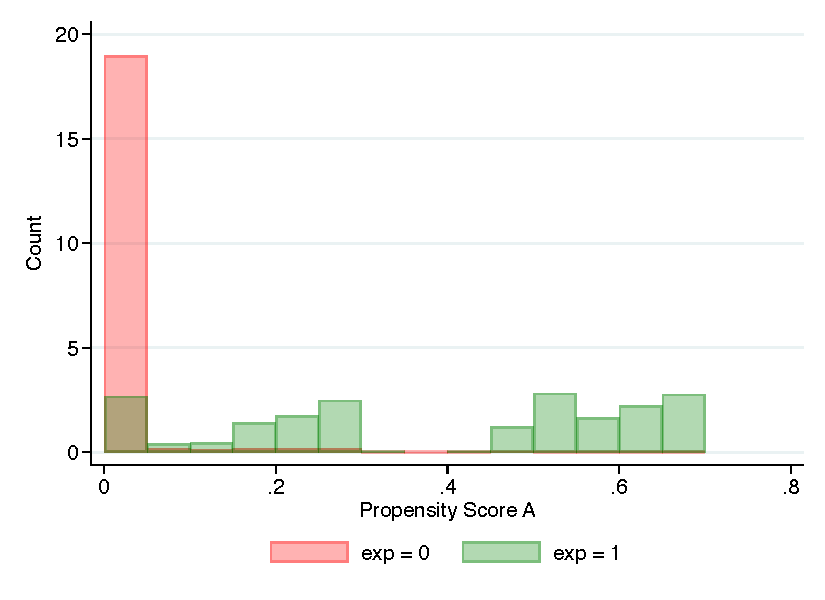
\includegraphics[width=11cm]{imgs/pscorea_hist.pdf}
\caption{Coarse score histogram, where $exp=0$ means data from CPS and $exp=1$ indicates experimental control data.}
\end{figure}

\begin{figure}[h]
\centering
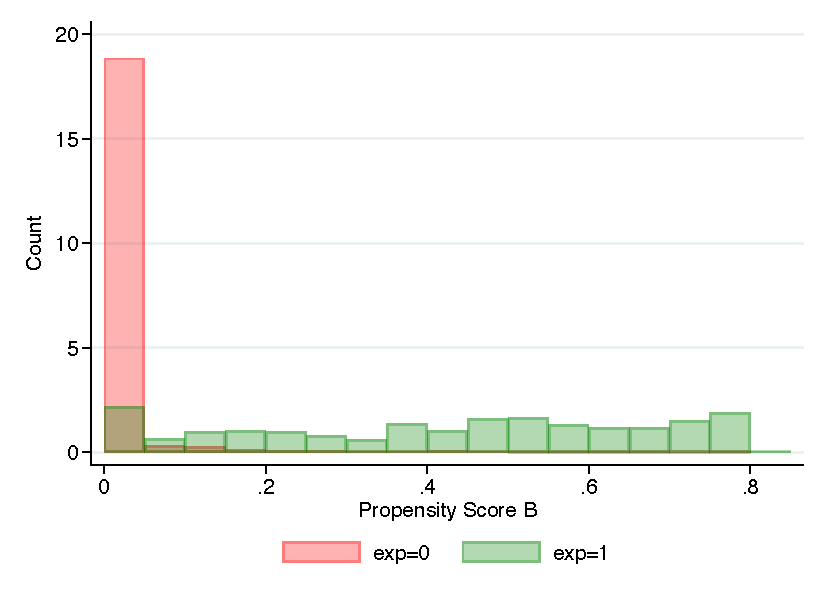
\includegraphics[width=11cm]{imgs/pscoreb_hist.pdf}
\caption{Rich score histogram, where $exp=0$ means data from CPS and $exp=1$ indicates experimental control data.}
\end{figure}

\hspace{0.41cm} \textbf{Question 9.} The kernel matching bias estimates are shown in Table 4 for the three bandwidths. The bandwidth with the smaller bias is 0.02, and the rest are greater the higher the bandwidth. In, general, all of this perform awfully, but the trend suggests that a smaller bandwidth will do a better job.

\begin{table}[h]
\centering
\begin{tabular}{lll}
\hline
bandwitdth & kernel M. & LLM   \\
\hline
0.02       & -2349   & -1981 \\
0.2        & -7043     & -2421 \\
2.0        & -9772     & 994  \\
\hline
\end{tabular}
\caption{Shows bias estimates for questions 9 and 10. }
\end{table}

\hspace{0.41cm} \textbf{Question 10.} The LLM bias estimates are shown in Table 4 for the three bandwidths. All of these bandwidths do a better job for LLM than for the kernel matching estimates. The bandwidth that yields a smaller bias in absolute value is 2.0. 

\hspace{0.41cm} \textbf{Question 11.} The coefficient of the OLS regression with rich covariates is -1853.39. This is in general better than the ones obtained with the matching methods, except for the LLM with bandwidth 2.0. Hence, we can conclude that the matching methods can yield better estimates. See results of regressions in the log file.  

\hspace{0.41cm} \textbf{Question 12.} Estimating the difference by the method proposed give a bias of -1851.5. This bias is pretty similar that the one obtained on the previous exercise. See details in the log file.  

\hspace{0.41cm} \textbf{Question 13.} The bias estimate without normalization is -1380. The bias estimate with normalization  is -1996. The first one presents a smaller bias but the second one should be theoretically desirable. See details in the log file.  

\end{document}